\documentclass{beamer}
\usepackage{relsize}
\usepackage{color}

\usepackage{listings}
\usetheme{CambridgeUS}
%\usepackage{beamerthemesplit} % new 
\usepackage{enumitem}
\usepackage{amsmath}                    % See geometry.pdf to learn the layout options. 
\usepackage{amsthm}                   % See geometry.pdf to learn the layout options. There 
\usepackage{amssymb}                    % See geometry.pdf to learn the layout options. 
\usepackage[utf8]{inputenc} 
\usepackage{graphicx}
\usepackage[english,bulgarian]{babel}

\lstset{language=C++,
                basicstyle=\ttfamily,
                keywordstyle=\color{blue}\ttfamily,
                stringstyle=\color{red}\ttfamily,
                commentstyle=\color{green}\ttfamily,
                morecomment=[l][\color{magenta}]{\#}
}

\newtheorem{mydef}{Дефиниция}[section]
\newtheorem{lem}{Лема}[section]
\newtheorem{thm}{Твърдение}[section]

\DeclareMathOperator{\restrict}{\upharpoonright}

\setitemize{label=\usebeamerfont*{itemize item}%
  \usebeamercolor[fg]{itemize item}
  \usebeamertemplate{itemize item}}

\setbeamercovered{transparent}



\begin{document}
\title[Увод в програмирането]{Структури} 
\author{Калин Георгиев} 
\frame{\titlepage} 

\section{Структури} 
\subsection{Идея}

\begin{frame}[fragile]
\frametitle{``Пакетиране'' на стойности}

\relscale{0.7}
\begin{lstlisting}
double distance (double x1, double y1, double x2, double y2)
{
  return sqrt ((x1-x2)*(x1-x2) - (y1-y2)*(y1-y2));
}

\end{lstlisting}	
\end{frame}


\begin{frame}[fragile]
\frametitle{``Пакетиране'' на стойности} 

\relscale{0.7}
\begin{lstlisting}
/*??????*/ western (double x1, double y1, double x2, double y2)
{
  if (x1 < x2)
    return /* (x1,y1) */;

   return /* (x2,y2) */;
}
\end{lstlisting}  

\end{frame}

\begin{frame}[fragile]
\frametitle{Структури} 


\begin{columns}[t]
  \begin{column}{0.3\textwidth}
      \relscale{0.7}
\begin{lstlisting}
struct Point  
{
  double x; //field x
  double y; //field y
}
\end{lstlisting}  

  \end{column}
  \begin{column}{0.7\textwidth}

\begin{itemize}
\item Дефиниране на променливи
\begin{flushleft}
\relscale{0.65}
\begin{lstlisting}
double a; 
int x,y;
Point p1, p2;
\end{lstlisting}  
\end{flushleft}

\item Достъп до полета
\begin{flushleft}
\relscale{0.65}
\begin{lstlisting}
p1.x = 10;
cout << p1.x;
p1.x = p2.x + 5;
\end{lstlisting}  
\end{flushleft}


\item Връщане като резултат
\begin{flushleft}
\relscale{0.65}
\begin{lstlisting}
Point western (Point p1, Point p2)
{
  if (p1.x < p2.x)
    return p1;
  return p2;
}
\end{lstlisting}  
\end{flushleft}


\end{itemize}


  \end{column}
\end{columns}



\end{frame}



\begin{frame}[fragile]
\frametitle{Пример} 

\relscale{0.7}
\begin{lstlisting}
Point western (Point p1, Point p2)
{
  if (p1.x < p2.x)
    return p1;
  return p2;
}

int main ()
{
  Point p1,p2;
  cin >> p1.x >> p1.y >> p2.x >> p2.y;

  Point p3 = western (p1,p2);
  cout << "The western point is (" 
       << p3.x 
       << ","
       << p3.y
       << ")" << endl;

  //cout << p3 ???
}

\end{lstlisting}  

\end{frame}

\begin{frame}[fragile]
\frametitle{Пример: Рационални числа} 

\relscale{0.7}
\begin{lstlisting}
sturct Rational
{
  double nom, denom;
};
\end{lstlisting}  
\flushright{$\frac{a_{nom}}{a_{denom}}+\frac{b_{nom}}{b_{denom}}=\frac{a_{nom}*b_{denom}+b_{nom}*a_{denom}}{a_{denom}}$}

\relscale{0.7}
\begin{lstlisting}
Rational sum (Rational a, Rational b)
{
  Rational result;
  result.nom = a.nom*b.denom + b.nom*a.denom;
  result.denom = a.denom * b.denom;
  return result;
}

Rational multiply (Rational a, Rational b)
{
  Rational result;
  result.nom = a.nom*b.nom;
  result.denom = a.denom*b.denom;
  return result;
}

void print (Rational a)
{
  cout << a.nom << "/" << a.denom;
}


\end{lstlisting}  

\end{frame}


\begin{frame}[fragile]
\frametitle{Пример: Рационални числа} 


\center{\relscale{1.5}{$a*b + c$}}
\relscale{0.7}
\begin{lstlisting}
double an,ad,bn,db,cn,cd;
//...
cout << an*bn*cd + cn*ad*bd;
     << "/"
     << ad*bd*cd;
\end{lstlisting}  

\begin{itemize}
  \item Алтернативно:
\end{itemize}


\begin{lstlisting}
Rational a,b,c;
//...
print (sum (multiply (a,b) , c));
\end{lstlisting}  

\end{frame}


\begin{frame}[fragile]
\frametitle{По-сложни примери} 

\begin{columns}[t]
  \begin{column}{0.4\textwidth}

\relscale{0.7}
\begin{lstlisting}
struct Date
{
  int day, month, year;
};
struct Person
{
  char name[100];
  Date birthdate;
};
\end{lstlisting} 
\relscale{1}

  \end{column}
  \begin{column}{0.6\textwidth}
\pause
\relscale{0.7}
\begin{lstlisting}
void readPerson (Person& p)
{
  cout << "Please enter name:";
  cin.getline (p.name,99);
  cout << "Please enter day, month,"
       << " and year:";
  cin >> p.birthdate.day 
      >> p.birthdate.month 
      >> p.birthdate.year;
}
void printPerson (Person p)
{
  cout << "Name:" << p.name 
       << " birthdate: " 
       << p.birthdate. day << "/" 
       << p.birthdate.month << "/"
       << p.birthdate.year << endl;
}

\end{lstlisting}  
  \end{column}
\end{columns}

 

\end{frame}


\begin{frame}[fragile]
\frametitle{Помощна функция} 

\relscale{0.7}
\begin{lstlisting}
bool earlier (Date d1, Date d2)
{
  if (d1.year < d2.year) return true;
  if (d1.year == d2.year && 
      d1.month < d2.month) return true;
  if (d1.year == d2.year && 
      d1.month == d2.month && 
      d1.day < d2.day) return true;

  return false;
}

\end{lstlisting}  

\end{frame}


\begin{frame}[fragile]
\frametitle{Масив от структури} 

\relscale{0.7}
\begin{lstlisting}

Person findYoungest (Person people[], int n)
{
  int index = 0;
  for (int i = 1; i < n; i++)
    if (earlier (people[i].birthdate,people[index].birthdate))
      index = i;
  return people[index];
}


\end{lstlisting}  

\end{frame}


\begin{frame}[fragile]
\frametitle{Група от хора} 


\begin{lstlisting}
Person people[10];
int i;

for (i=0; i<10; i++)
  readPerson (people[i]);

printPerson (findYoungest (people,10));

\end{lstlisting}  

\end{frame}
 

\subsection{Представяне} 

\begin{frame}
\centerline{Представяне в паметта}
\end{frame}


\begin{frame}[fragile]
\frametitle{Представяне в паметта} 

\begin{figure}
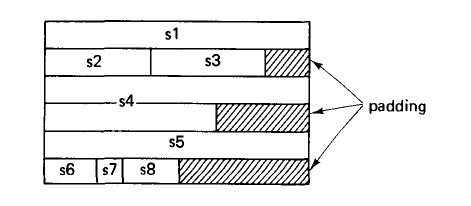
\includegraphics[width=8.5cm]{images/padding}
\caption{Подравняване (padding)\cite{wirth}}  
\end{figure}

\end{frame}


\begin{frame}[fragile]
\frametitle{Представяне в паметта} 


\begin{columns}[t]
  \begin{column}{0.7\textwidth}
  
  \begin{flushleft}
  
  \relscale{0.5}
  
\begin{lstlisting}
struct S {Ta a; Tb b; Tc c;};
S x;
\end{lstlisting}
   \end {flushleft}

\begin{itemize}
\item \textbf{НЕ МОЖЕМ} да разчитаме, че:
\end{itemize}

\begin{flushleft}
\relscale{0.8}
\begin{lstlisting}
sizeof (S) == sizeof (Ta) + sizeof (Tb) + sizeof (Tc)
(long)&x.b == (long)&x + sizeof (Ta);
\end{lstlisting}
\end{flushleft}

  \end{column}
  \begin{column}{0.3\textwidth}
\begin{figure}
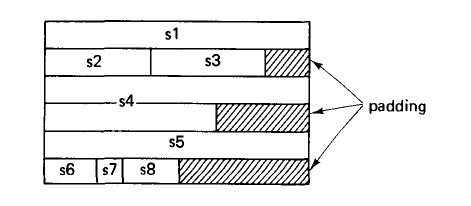
\includegraphics[width=4.5cm]{images/padding}
\end{figure}

  \end{column}
\end{columns}


\end{frame}


\begin{frame}
\centerline{Указатели и функции}
\end{frame}


\begin{frame}[fragile]
\frametitle{Указатели} 


\begin{columns}[t]
  \begin{column}{0.7\textwidth}

\begin{flushleft}
\relscale{0.8}
\begin{lstlisting}
double *pb = &x.b; //double*
*pb = 10;
cout << *pb << x.b;

S arr[10];
pb = &arr[3].b;
*pb = 10;
cout << *pb << arr[3].b;

S* ps = &art[3];
ps->b = 15;
cout << ps->b 
     << (*ps).b 
     << arr[3].b;

\end{lstlisting}
\end{flushleft}
  \end{column}
  \begin{column}{0.3\textwidth}

\begin{flushleft}
\relscale{0.6}
\begin{lstlisting}
struct S 
{
  int a; 
  double b; 
  char c;
};
S x;
\end{lstlisting}
\end{flushleft}


  \end{column}
\end{columns}



\end{frame}




\begin{frame}[fragile]
\frametitle{Функции} 


\begin{columns}[t]
  \begin{column}{0.6\textwidth}

\begin{flushleft}
\relscale{0.8}
\begin{lstlisting}
void f (S z)
{
  cout << z.b; 
  z.b = 10; 
  cout << z.b;}

void g (S& z)
{cout << z.b; z.b = 20;}

void h (S* z)
{z->b = 30;}

S i (S z)
{cout << z.b; z.b = 40; return z;}

\end{lstlisting}
\end{flushleft}
  \end{column}
  \begin{column}{0.4\textwidth}

\begin{flushleft}
\relscale{0.8}
\begin{lstlisting}
int main ()
{
  S x;
  x.b = 0;

  f(x); cout << x.b;
  g (x); cout << x.b;
  h (&x); cout << x.b;
  

  cout << i(x).b;
  cout << x.b;
}
\end{lstlisting}
\end{flushleft}


  \end{column}
\end{columns}



\end{frame}



\textbf {Библиография}
\begin{thebibliography}{9}

\bibitem{wirth} Niklaus Wirth.  \emph{``Algorithms + Data Structures = Programs''},Prentice-Hall Series in Automatic Computation, 1976

\end{thebibliography}






\end{document}




\begin{columns}[t]
  \begin{column}{0.2\textwidth}

\relscale{0.63}
\begin{lstlisting}
\end{lstlisting}
\relscale{1}

  \end{column}
  \begin{column}{0.8\textwidth}

  \end{column}
\end{columns}

